\documentclass[preprint]{aastex} %double-column, single-spaced document:
%\documentclass[iop,floatfix]{emulateapj} 

\usepackage{hyperref}
%\usepackage{graphicx}
%\usepackage{apjfonts}
\usepackage{enumerate}
\usepackage{amsmath,amssymb}
\usepackage{geometry}
\usepackage{bm}

\newcommand{\prob}{{\rm prob}}
\newcommand{\qN}{\{q_i\}_{i=1}^N}
\newcommand{\qM}{\{q_{im}\}_{i=1,m=0}^{N,M}}
\newcommand{\yN}{\{y_i\}_{i=1}^N}
\newcommand{\vt}{\vec{\theta}}
\newcommand{\vg}{\vt_{\star, {\rm grid}}}
\newcommand{\vpp}{\vt_{\star, {\rm post}}}
\newcommand{\vstar}{\vt_{\star}}
\newcommand{\vN}{\vt_{\rm N}}
\newcommand{\vc}{\vec{c}}
\newcommand{\fM}{ {\bm M}}
\newcommand{\fMi}{M_i}
\newcommand{\fD}{ {\bm D}}
\newcommand{\fDi}{D_i}
\newcommand{\dd}{\,{\rm d}}
\newcommand{\trans}{\mathsf{T}}
\newcommand{\Z}{[{\rm Fe}/{\rm H}]}
\newcommand{\A}{[\alpha/{\rm Fe}]}

%\slugcomment{}
%\shorttitle{}
%\shortauthors{}

\begin{document}

\title{Methods for the spectroscopic inference of fundamental stellar parameters}
\author{\today{}\\
\medskip
Ian~Czekala\altaffilmark{1} et al.
%Author2\altaffilmark{2},
}

\altaffiltext{1}{Harvard-Smithsonian Center for Astrophysics, 60 Garden Street MS 10, Cambridge, MA 02138}
%\altaffiltext{2}{Institution 2}
\email{iczekala@cfa.harvard.edu}

\section{Introduction}
The fundamental properties of stars---effective photospheric temperature, surface gravity, and metallicity--are crucial for our understanding of pre-main sequence stellar evolution \citep{dm97, bca+02}. The exoplanet community is also intensely focused on deriving accurate stellar properties because the properties of newly discovered exoplanets must necessarily be quoted relative to those of their host stars (e.g. \citealt{tfs+12,blj+12,ssm+13}) and uncertain star properties translate into uncertain planet properties \citep{kan14}. Many techniques\footnote{If you are interested, I have also compiled a more verbose review of modern techniques described in the literature. However, for the sake of brevity I have omitted it from this document.} exist for stellar characterization such as line indexes, machine learning, and spectral synthesis\footnote{Given infinite computational power, we would prefer to fit \emph{all} of the parameters that completely describe a synthetic spectrum: atmospheric structure, individual elemental abundances, and atomic constants describing the opacity contribution of a line. Approximations to the synthesis and efficient MCMC sampling parallelized on a cluster might soon put this approach within reach.}. In order to derive accurate and robust stellar properties for our small sample ($\sim 20$) of T Tauri stars (some binary), we have decided to forward model the observed spectra by drawing from a grid of synthetic spectra.

\begin{table}[!htb]
\begin{tabular}{ll}
\hline
\hline
Symbol & Description\\
\hline
\hline
$i$ & index specifying a pixel\\
$\lambda_i$ & wavelength corresponding to a given pixel $i$\\
$\vg$ & fundamental stellar parameters, $T_{\rm eff}, \log(g), \Z, \A$\\
  & that parameterize a synthetic spectrum from the grid\\
$\vpp$ & stellar parameters $v \sin i$, $v_z$, $A_V$, and $R^2/d^2$ that\\
  & are applied during ``post processing'' of the synthetic spectrum\\
$\vstar$ & $\{\vg,\vpp \}$\\
$c_0, c_1, \ldots$ & Chebyshev polynomial coefficients for residual flux calibration\\
$\vN$ & the set of nuisance parameters composed of $\{c_0, c_1, \ldots, c_N\}$\\
$k(i | \vN)$  & polynomial function that multiplies a synthetic spectrum\\
$\vt$ & the parameters $\{\vg, \vpp, \vN\}$ that completely describe a model spectrum\\
$\fDi$ & data flux for a given pixel, $D(\lambda_i)$\\
$\fD$ & data vector comprised of all $\fDi$, $i = \{0, \ldots, N\}$\\
$\fMi$ & model flux for a given pixel, $M(\lambda_i | \vt)$\\
$\fM$ & model vector comprised of all $\fMi$, $i = \{0, \ldots, N\}$\\
$\sigma_i$ & Poisson noise for a given pixel $i$\\
$R_i$ & residuals $(\fDi - \fMi)/\sigma_i$\\
\hline
\end{tabular}
\caption{Nomenclature used in this document}
\label{tab:nomenclature}
\end{table}

\subsection{Pixel to pixel techniques using synthetic spectral libraries}
\label{sec:pix}
Most forward modeling techniques compare pixels directly using some form of
\begin{equation}
  \chi^2 = \sum_i \left [\frac{ \fDi - \fMi}{\sigma_i} \right ]^2 = \sum_i R_i^2
\end{equation}
where the variables are defined in Table~\ref{tab:nomenclature}. A serious problem with this approach is that synthetic spectra are not perfect: systematic errors invalidate the $\chi^2$ assumption and bias parameter estimates and their uncertainties.

Current methods either circumvent this problem by using high quality synthetic grids that were painstakingly tuned over a narrow wavelength range \citep[$\lesssim 500$ \AA]{blj+12,sb13}, or they use less-perfect grids with full optical coverage and sigma clip the bad regions of the spectrum \citep{kpb+09,mga13}. Masking (either implicitly or explicitly, respectively) is troublesome because, in the words of \citet{mga13}, ``regions with [only] modest agreement between the real and synthetic spectra [that might be masked] may contain more temperature information than regions with slightly better matches, and we have no a priori information about what spectral regions are the most temperature sensitive.'' Masking could very well destroy stellar information in the pursuit of a better fit. 

\begin{figure}[!htb]
\begin{center}
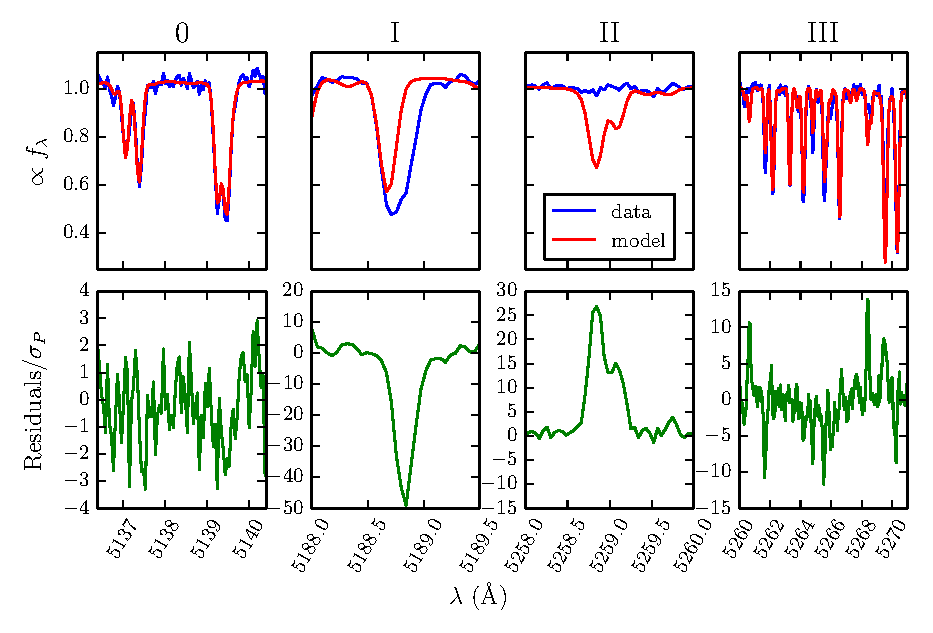
\includegraphics{lineclasses}
\caption{The four classes of line behavior. \textbf{Class 0}: the model behaves as expected. \textbf{Class I}: a spectral line is present in the data but missing from the model (in this case, the line is also blended). \textbf{Class II}: a spectral line exists in the model where there is only continuum in the data. \textbf{Class III}: lines exist in both the data and model, but some are too strong while others are too weak. The lower panels show the residual spectra in units of the Poisson uncertainty. The data is a spectrum of WASP-14, an F star. The model is from the PHOENIX grid\citep{hwd+13}.}
\label{fig:lineclasses}
\end{center}
\end{figure}

\subsection{Classes of synthetic spectral line behavior}
Illustrated in Figure~\ref{fig:lineclasses} are three ways that synthetic spectra often diverge from reality. When a spectral line appears in the data but not in the model, due to interstellar or telluric absorption or a missing opacity source, we call this a \textbf{Class I} error. When a spectral line appears in the model but not in the data, presumably due to a combination of incorrect atomic constants or atmospheric structure, we label it a \textbf{Class II} error. Both of these types of errors are present over a wide range of probable stellar parameters (1000 K in $T_{\rm eff}$, and 1 dex in $\log(g)$, $\Z$, and $\A$) and there does not exist a $\vg$ that could ever fit these lines, making these regions useless for determining stellar parameters. We know that for a normal AFGK star Class I residuals will always be negative and will not change significantly with $\vg$, while Class II residuals will always be positive and their magnitude should decrease with decreasing metallicity. To help identify Class I and II errors,  we could use the partial derivatives of an individual synthetic spectrum with respect to $\vg$ and a prior on the range of parameters over which the residuals will be correlated to determine which lines show Class I or II behavior.

When some line strengths do not match at a $\vg$ that properly fits most other lines, we term these \textbf{Class III} errors. These types of errors are pernicious because there does exist a $\vg$ that would fit each line individually, but no one $\vg$ can be chosen that fits all the lines. We must then decide which regions to trust and by how much, because Class III regions \emph{still contain information about $\vg$}. In fact, they might contain \emph{the most} information about $\vg$ since these delicate regions are the most sensitive to changes in $\vg$ and are consequently whey they are the hardest to model correctly. In other words, Class III regions might be where the spectrum gradient ($\sum_{j} \partial \fMi/ \partial \vt_{ \star {\rm grid}, j}$) is the largest. 

\section{In the limit of a perfect stellar model}
To generate a model spectrum $\fM(\vg, \vpp)$, we use $\vg$ to linearly interpolate a synthetic spectrum from the grid, and then use $\vpp$ to apply instrumental and rotational broadening in the Fourier domain, Doppler shift, correct for extinction, and then downsample to the exact pixels of the data spectrum using spline interpolation\footnote{Because we are dealing with flux-calibrated data and synthetic spectra, we \emph{resample} to lower resolution. We do not \emph{rebin} because we are dealing with flux-density, not photon counts}.

To account for imperfect flux calibration, we extend the approach of \citet{elh+06} and multiply $\fM(\vg, \vpp)$ by $k(\vN)$, which is a Chebyshev polynomial described by a set of $N$ Chebyshev coefficients. We can either sample in the coefficients or analytically marginalize over them. We favor this approach over the traditional technique of normalizing to the stellar continuum due to concerns about correctly placing the pseudo-continuum in M stars. From now on we refer to $\fM(\vt) = k(\vN) \fM(\vg, \vpp)$. The mathematical details are in \S~\ref{sec:chebyshev}.

Currently we are sampling this $\chi^2$ posterior with the MCMC ensemble sampler \citep{gw10} implemented in \texttt{Python} by \citet{fhl+12} as \texttt{emcee}. In this section, we described our approach to sample the posterior assuming perfect synthetic spectra. However, if one does a straight up $\chi^2$ fit to our spectra, one can get posteriors that have 1-sigma contours of $\pm 1$ K and $\pm 0.01$ dex in gravity and metallicity. This would be as precise as stellar parameters obtained with astroseismology! Clearly there is something going wrong here.

\section{Beyond a perfect stellar model}
\label{sec:residuals}
\subsection{Additional sources of noise}
\begin{itemize}
  \item CCD readnoise and imperfect 1D spectrum extraction over night sky lines will almost definitely increase the noise in a pixel beyond theoretical Poisson limits. Normally this information will be encapsulated in a ``sigma spectrum'' output by IRAF, but unfortunately we do not have access to this for our current dataset.
  \item The stellar continuum can flicker/jitter (as shown by Kepler), which would produce a small departure from a perfect continuum. This might explain why even in the Class 0 region of our spectrum (Figure~\ref{fig:lineclasses}, left panel) the residuals are slightly larger than 1 $\sigma$ on average. For our T Tauri stars this effect may be more pronounced.
  \item When we interpolate a synthetic spectrum from the library to a specific $\vg$, we will introduce interpolation errors depending on how close we are to a grid point in the library. \citet{hus12} investigate the possible range of interpolation errors at specific $\vg$ by dropping out a spectrum from the grid, interpolating over it, and then comparing the true spectrum to the interpolated spectra. For hotter stars with well defined continua, we find the maximum error is $\lesssim 5$\%, while for M stars the error could be as large as $\sim 20$\% for some spectral features. By doing this interpolation test across the grid, we could determine an ``interpolation error spectrum'' that would encapsulate the maximum error possible for an interpolated spectrum, weighted by its distance from the nearest grid points. If a typical spectrum has signal/noise of $\sim 30$ per pixel (or noise/signal ratio of $1/30 \approx 3$\%), an interpolation noise contribution of $\sim 5$\% the level of the signal level would be significant. 
\end{itemize}
However, we have tried arbitrarily increasing the Poisson errors by a factor of 2 or 3 and it didn't significantly change the results, suggesting that something more drastic is needed beyond simply adding in more noise.

\subsection{Gallery of likelihood functions}
\label{sec:gal}
A problem with the $\chi^2$ likelihood function is that the Gaussian tails rapidly decline, making outliers extremely improbable. A common approach for ``robust regression'' is to use a likelihood function with fatter, more forgiving, tails. Although not rigorously motivated, this is can be a quick thing to try. We explored several likelihood functions including a combination of Gaussian with exponential wings, a Lorentzian (Cauchy) function, and a function described  by \citet{ss06}, which treats the noise estimate for each data point suspiciously. In Sivia's model, the true noise $\sigma$ can be no smaller than some original estimate $\sigma_0$, but it may be much larger. By putting a prior on $\sigma$, 
\begin{equation}
  p(\sigma_i | {\sigma_0}_i) = \left \{ \begin{array}{cc}
    {\sigma_0}_i/\sigma_i^2 & \sigma_i  \leq {\sigma_0}_i\\
    0                 & \textrm{else}
  \end{array}
    \right.
\end{equation}
and marginalizing over the $\chi^2$ likelihood, the new likelihood function becomes
\begin{equation}
p(\fDi | \fMi, {\sigma_0}_i) = \frac{1}{ {\sigma_0}_i \sqrt{2 \pi}} \left [ \frac{1 - e^{-R_i^2/2}}{R_i^2} \right ] 
\end{equation}
where $R_i = (\fDi - \fMi)/{\sigma_0}_i$. This function has even fatter tails than the exponential model and seems to give results less biased by outliers, however it is not truly satisfying. Which lines contributed most to the posterior? What about the wings of class I and II errors? These individual pixels might still be given a weight of ${\sigma_0}_i$ because they are not nearly as bad as the line centers.

Other functions we might try in the future include a Student-$t$ distribution, a linear combination of Gaussians, or the $\chi^2_Q$ function described in \citet{hbl10}. While ``softer'' likelihood functions do help somewhat, we would like to move beyond tweaking the fitting function towards an approach that properly incorporates our knowledge of the systematic errors of the synthetic grids. In the remaining two sections of this document we outline potential ideas that we might try next, but have not yet implemented in code.

\section{Bad data mixture model}
The bad data model \citep{pre97,hbl10} is a powerful framework for forward modeling data, which allows the modeler to explicitly account for outliers using a generative model. In the simplest mixture model, each pixel has a binary flag $q_i$ which specifies whether that data point is good or bad. Then, for the entire data set we have an ensemble of $\qN$. If this ensemble of $\qN$ is chosen appropriately, and the good pixels are flagged as good and the bad pixels are flagged as bad, the posterior will be maximized. We adopt $P_B$ for the \emph{a priori} probability that a given pixel will be bad, $Y_b$ for the mean flux of the bad pixels, and $V_b$ for their variance. Written out explicitly, this is
\begin{multline}
  {\cal L} = p({\bm D} | \vt,\qN, Y_b,V_b) = \prod_{i=1}^N \left [ \frac{1}{\sqrt{2 \pi} \sigma_i} \exp \left[ - \frac{(\fDi - \fMi)^2}{2 \sigma_i^2} \right] \right ]^{q_i}  \times \\
  \left [ \frac{1}{\sqrt{2 \pi (V_b + \sigma_i^2)}} \exp \left[ - \frac{(\fDi - Y_b)^2}{2 (V_b + \sigma_i^2)} \right]
  \right ]^{1 - q_i}
\end{multline}
If we put a Bernoulli prior on the $q_i$
\begin{equation}
  p(q_i | P_b) = [1-P_b]^{q_i} P_b^{[1-q_i]}
\end{equation}
the probability of any given ensemble of $\qN$ is 
\begin{equation}
  p(\qN | P_b) = \prod_{i=1}^N [1-P_b]^{q_i} P_b^{[1-q_i]}
\end{equation}
We can analytically marginalize over the settings for a single flag by a discrete sum over the two states of $q_i = 1$ and $q_i = 0$. 
\begin{multline}
  p(\vt, P_b, Y_b, V_b | D_i)  =  \int p( \vt, q_i, P_b, Y_b, V_b| D_i) {\rm d} q_i \\
  = p(\vt, q_i=1, P_b, Y_b, V_b | D_i) + p(\vt, q_i=0, P_b, Y_b, V_b | D_i) \\
  = \Bigl[ p_{\rm good}(D_i | \vt)\, p(q_i=1 | P_b) +  p_{\rm bad}(D_i | Y_b, V_b)\, p(q_i=0 | P_b)\Bigr] \times p(\vt ,P_b, Y_b,V_b) 
\end{multline}

\begin{multline}
  p(\vt,P_b,Y_b,V_b|\,{\bm D}) \propto \prod_{i=1}^N \Bigl [ [1 - P_b] p_{\rm good}(D_i |\vt)  + P_b p_{\rm bad}(D_i | Y_b, V_b)\Bigr ] \times p(\vt,P_b, Y_b, V_b)\\
  \boxed{
    = \prod_{i=1}^N \left\{ \frac{1 - P_b}{\sqrt{2 \pi \sigma_i^2}} \exp \left[ - \frac{(\fDi - \fMi)^2}{2 \sigma_i^2} \right] + \frac{P_b}{\sqrt{2 \pi (V_b + \sigma_i^2)}} \exp \left[- \frac{(\fDi - Y_b)^2}{2 (V_b + \sigma_i^2)} \right] \right\}
  \times p(\vt,P_b,Y_b,V_b)}
\end{multline}

In its simplest form, the bad data model results in a likelihood function that is a linear combination of Gaussians. Although this functional form might be similar to some of the likelihood functions in \S~\ref{sec:gal}, the benefit of this bad data approach over a gallery of likelihood functions is that it is motivated by the characteristics of the bad data ($P_B$, $Y_b$, and $V_b$). If we wish to add additional information about the characteristics of the bad data, we can do so. 

\subsection{Mixture of multiple components}
When we believe that a sample population might be composed of several populations with different behaviours (Class 0, I, II, and III), we can expand the bad data model to a multiple mixture model. Following \citet{gcs+04}, we develop a mixture model with $M=4$ components, one for each class of error. Our likelihood function is then
\begin{equation}
  p(\fD, \vec{Q} | \vt, J) = \prod_i^N \prod_{m=0}^M \left [ J_m {\cal L}_m(\fDi | \vt_m) \right ]^{q_{im}}
\end{equation}
where $\vec{Q} = \qM$ is a two dimensional array ($N \times M$) of all the individual $q_{im}$ flags, and $J_m$ is a weight that represents the total fraction of each component in the mixture\footnote{The weights are normalized $\sum_m J_m = 1$}, and ${\cal L}_m$ is the likelihood function for $m$th mixture component. At this point, $\vt$ now contains all of the parameters that might be used by any of the likelihood functions. $\vt_m$ is used to denote only those parameters that will be used for ${\cal L}_m$. Given what we know about these synthetic spectral errors, we could specify the following likelihood functions
\begin{equation}
  \begin{array}{lcccc}
 {\cal L}_0 &= p(\fDi, q_{i0} = 1) &\rightarrow & \textrm{Class 0} & \chi^2\\
 {\cal L}_1 &= p(\fDi, q_{i1} = 1) &\rightarrow & \textrm{Class 1} & \textrm{flat lnprob}\\
 {\cal L}_2 &= p(\fDi, q_{i2} = 1) &\rightarrow & \textrm{Class 2} & \textrm{flat lnprob}\\
 {\cal L}_3 &= p(\fDi, q_{i3} = 1) &\rightarrow & \textrm{Class 3} & \textrm{soft } \chi^2\\
\end{array}
\end{equation}
This would treat Class I and II errors as if they had been masked from the dataset but allow Class III to have a slight influence on the posterior since these regions still contain information about $\vstar$. The softening term of the $\chi^2$ could even be sampled for, much like the $V_b$ of the original bad data model.

\subsection{Spatial correlations of pixels}
Previously we assumed that each data point is independent, but we know that the spectrum is spatially correlated across several pixels with a correlation length set by the width of the convolution of the stellar rotation kernel ($v \sin i$) and the instrumental resolution kernel, which is also the typical width of a spectral line\footnote{Some very strong lines (such as the Balmer lines or Mg b triplet) will have wings with a larger correlation length.}. This correlation length will have some dependence on the spectral type of star. For example, F and G stars will likely have singular, well-defined lines while M stars might have a large molecular feature covering a wide swath of the spectrum. Neighboring pixels are actually correlated in two coordinates: the $q_{im}$ flags and the residuals $R_i$. 

\subsubsection{Correlation of the $q_i$ flags}
The pixels at the center of a bad line will give a strong residual response, which will likely be flagged as bad. However, the pixels in the wings of the spectral line might not be sufficiently egregious to be properly flagged. To remedy this situation, we attempt to develop a bad data model which includes spatial (wavelength) correlations.

In the manner of Gaussian random processes (GRP), we develop a covariance function
\begin{equation}
  {\rm cov}(q_i, q_j) = \rho(| i - j|)
\end{equation}
\begin{equation}
  \Sigma_{ij} = \sigma^2 \rho(|i - j|)
\end{equation}
that describes the correlation between the state of the bad data flags. The simplest thing to do would be to assume a common correlation length in the spectrum. If we say that the typical feature will have three contiguous pixels\footnote{Ideally the covariance function should be a function over $\lambda_i$ in velocity space, since all spectral features should have a similar velocity width. For the purpose of keeping the math simple for the moment, we use pixel index and assume the pixels are uniformly spaced.} wrong, then the correlation function would be
\begin{equation}
  {\rm cov}(q_i, q_j) = \left \{ \begin{array}{cc}
    1 - \frac{|i - j|}{3} & |i - j| < 3 \\
    0                                    & \textrm{else}
\end{array}
\right .
\end{equation}
and the matrix would be
\begin{equation}
  \begin{bmatrix}
    1 & 2/3 & 1/3 & 0 & \cdots & 0\\
    2/3 & 1 & 2/3 & \ddots & \ddots & \vdots\\
    1/3 & 2/3 & \ddots & \ddots & \ddots & 0\\
    0  & \ddots & \ddots & \ddots & 2/3 & 1/3\\
    \vdots & \ddots & \ddots & 2/3 & 1 & 2/3\\
    0      & \cdots & 0 & 1/3 & 2/3 & 1\\
  \end{bmatrix}
\end{equation}
Because our correlation function has compact support, we now have a sparse covariance matrix. This can potentially speed up a matrix computation that would otherwise be very slow. 

\subsubsection{Correlation of adjacent residuals}
Not only will the flags $q_i$ be spatially correlated but so will the values of the residuals $R_i$. For OBAFGK stars, the residuals are likely to be shaped like Gaussians. If $i$ specifies the pixel at the line center of a large residual feature, then the neighboring $i \pm 1,2,\ldots$ pixels will have also have similar residuals but of declining magnitude $|R_{i\pm 1, 2, \ldots} | \lesssim |R_i|$.  For M stars, there might be a wider correlation length and the shape of the lines might not be well-described by a Gaussian. 

I am new to the field of GRP, but it seems like it might be possible to come up with a covariance function that would describe the predicted heights of the residuals and regress against them. The covariance function between $R_i$ could be learned from the spectrum itself. Then, the likelihood functions for each mixture component in the model would be custom tailored for the type of error that it expected to encounter. For example, Class 0 residuals would be flat while Class I, II, and III residuals would have some sort of Gaussian shape. Class I residuals would be negative while Class II residuals would be positive. I plan to further investigate covariance functions. 

\subsubsection{Further ideas}
\begin{itemize}
  \item \citet[ch. 18]{gcs+04} list several references further describing inference for spatially-correlated data and I plan to work my way through these. 
  \item Naively, it seems to me like there might be a way to use FFT methods to help speed up the correlation calculation, similar to Gaussian random fields.
  \item My preliminary experiments with GRP reveal that there is an art in choosing the functional form of ${\rm cov}(i, j)$ and setting the hyperparameters. Perhaps these could also be parameters that we sample in. I am working through \citet{rw05} and \citet[Ch 21.]{gcs+13} to learn more.
\end{itemize}

\subsection{Hyperparameters}
\citet{mb13} discuss a technique to deal with systematic errors when combining different data sets for the combined inference of a single problem. They use a hyperparameter approach that can artificially inflate the variance of each data set to find a common posterior and allow for correlations between data sets. We could set up a similar hyperparameter approach that can tune the likelihood contribution for certain lines, treating each line as they do different datasets. If all of the lines were in harmonious agreement, this hyperparameter would undergo ``shrinkage'' \citep{kru10} and tighten the posterior on $\vstar$. If the line fits were incompatible, this hyperparameter would increase while also broadening our posterior on $\vstar$.

\subsection{Sampling ideas for the mixture model with spatial correlations}
If we use multidimensional Gaussian likelihood functions and correlation functions with compact support, it might still be possible to analytically marginalize over the multiple mixture components. If we cannot marginalize, then we need alternate sampling methods to explore the parameter space in a computationally efficient manner. A stellar model with flags for each pixel would have $\vstar + (N \times M)$ parameters, where for a typical high resolution optical spectrum $N >$ 100,000. 

An alternative way to approach this problem is to do Gibbs sampling where we propose a jump in a single $q_{im}$ at a time. Such a sample requires none of the previous heavy lifting (spectral grid interpolation, rotational broadening, or pixel interpolation), and so even though there are $\sim$ 100,000 flags to sample, this might be computationally feasible.

In order to ``trim the tree,'' \citet{gcs+04} suggest to start with a crude estimate (such as $k$-means clustering) to tentatively identify which observations have been drawn from which mixture components. They also suggest that the expectation-maximize (EM) algorithm could also be used to sample this posterior, although this is an algorithm that I need to research further.

\section{Injection of fake lines}
As an alternative approach to modeling the regions of the spectrum suffering from systematics, we could attempt to patch the models by injecting fake lines into the spectrum to compensate the errors. Each line could be a Gaussian parameterized by $\lambda_0$, strength, and FWHM. The line strength distribution could be described by a hyper prior, and the FWHM described by a hyper parameter, since all lines should have pretty much the same FWHM. We could penalize the model fits by having a prior on the number of bad lines that can be created. Given a bad line and the linelist that produced the synthetic models, it may be possible to identify other regions of the spectrum that might be bad. For example, if a vanadium line is bad, then we could check to see if the other vanadium lines might also be bad. 

Class III errors might be difficult to address in this paradigm since we would be fitting the difference of two lines, but if they are both Gaussians of the same FWHM, then it should still work. In M star spectra, rather than adding a Gaussian, we might need to add a larger continuum feature, which might be difficult to parameterize.

\subsection{Piecewise metallicity model}
In theory, it is possible to fit the profiles of only certain elements to determine the abundances of these elements. By masking all non-alpha elements, \citet{hus12} use PHOENIX spectra \citep{hwd+13} to derive alpha abundances of stars. Rather than masking, we could assemble a piecewise spectrum where regions of the spectrum might be drawn from a different combination of $\vg$, say with lower metallicity for some lines in order to account for a bad line strength. These regions would have to be normalized properly so that the composite spectrum is sufficiently smooth. Coupled with a linelist, one could also tweak individual elemental abundances.

\clearpage
\appendix
\section{A technique to account for imperfect flux calibration}
\label{sec:chebyshev}

The first four Chebyshev polynomials are 
\begin{align*}
  T_0(x) &= 1\\
  T_1(x) &= x\\
  T_2(x) &= 2 x^2 - 1\\
  T_3(x) &= 4 x^3 - 3x\\
\end{align*}
In our implementation, we map the full pixel range of a specific order $i \in [i_{\rm min}, i_{\rm max}]$ to $x \in [-1, 1]$. By mapping to pixel number rather than wavelength, we are insensitive to Doppler shifts of the model. If the spectrum has multiple orders, like echelle spectra, we would have a set of Chebyshev coefficients $\vN = \{ c_0, c_1, c_2, \ldots, c_N \}$ for each order.
\begin{align}
  k(i | \vN) &= c_0 T_0(i) \left [1 + c_1 T_1(i) + \ldots + c_N T_N(i) \right ]\\
  k(i | \vN) \fMi &=  \left [1 + \sum^N_{j = 1} c_j T_j(i) \right ] (c_0 \fMi)\\
  \label{eqn:k_new}
\end{align}
This functional form of $k$ allows $c_0$ to scale by large amounts while the higher order terms are perturbations on top of the \emph{scaled} model ($c_0 \fMi$). This formulation permits large rescalings up or down without biasing the higher order terms. If $c_0$ is expected to be small, we can use a simpler implementation described in \S\ref{sec:gaussian_simplification}. Then for the full spectrum   
\begin{equation}
  \ln \bigl [p(\vt | \fD) \bigr] \propto - \frac{1}{2} \sum_i \left [\frac{\fDi - \bigl [1 + \sum^N_{j = 1} c_j T_j(i) \bigr ] c_0 \fMi }{\sigma_i} \right ]^2
  \label{eqn:lnprob2}
\end{equation}
To simplify the following discussion, we consider a single pixel $i$ and then generalize this to a sum over all pixels later. We expand out the square in Equation~\ref{eqn:lnprob2}
\begin{equation}
  \ln \bigl [p(\vt | \fDi) \bigr] \propto - \frac{1}{2 \sigma_i^2} \left [ \fDi^2 - 2 \fDi c_0 \fMi \left [1+ \sum_{j=1}^N c_j T_j(i) \right ]+ c_0^2 \fMi^2 \left [1 + 2 \sum_{j=1}^N c_j T_j(i) + \sum_{j=1}^N \sum_{k=1}^N c_j T_j(i) c_k T_k(i) \right ] \right ]
  \label{eqn:expanded}
 \end{equation}
To simplify the notation, we can rewrite the higher order Chebyshev coefficients and polynomials as column vectors $\vc$ and $\vec{T}(i)$, respectively
\begin{equation}
  \vc = 
  \begin{bmatrix}
    c_1\\
    c_2\\
    \vdots\\
    c_N
  \end{bmatrix}
  \hspace{3cm}
\vec{T}(i) = 
\begin{bmatrix}
T_1(i)\\
T_2(i)\\
\vdots\\
T_N(i)\\
\end{bmatrix}
\end{equation}
then 
\begin{equation}
  k(i| \vN) = c_0 \left [ 1 + \sum^N_{j = 0} c_j T_j(i) \right ] = c_0 \left[ 1+ \vec{T}^\trans \cdot \vc \right]
\end{equation}
If we let 
\begin{equation}
  {\bm W}(i) = \vec{T} \cdot \vec{T}^\trans = 
  \begin{bmatrix}
T_1 T_1 & T_1 T_2 &  \hdots & T_1 T_N \\
T_2 T_1 & T_2 T_2 &  \hdots & T_2 T_N \\
\vdots  & \vdots  &  \ddots & \vdots \\
T_N T_1 & T_N T_2 &  \hdots & T_N T_N \\
  \end{bmatrix}
\end{equation}
then we have
\begin{equation}
  \sum_{j =1}^N \sum_{k=1}^N c_j T_j(i) c_k T_k(i) = \vc^\trans \cdot {\bm W} \cdot \vc
\end{equation}
We can rewrite Equation~\ref{eqn:expanded} quadratically in $\vc$ as
\begin{equation}
  \ln \bigl [p(\vt | \fDi) \bigr] \propto - \frac{1}{2} \frac{c_0^2 \fMi^2}{\sigma_i^2}  \vc^\trans {\bm W} \vc + \left (\frac{- c_0^2 \fMi^2 + c_0 \fDi \fMi}{\sigma_i^2} \right ) \vec{T}^\trans \vc -  \left( \frac{c_0^2 \fMi^2 - 2 c_0 \fDi \fMi + \fDi^2}{2 \sigma_i^2} \right)
\end{equation}
Because matrix multiplication is associative, we can sum ${\bm W(i)}$ and $\vec{T}^\trans(i)$ across all pixels and define
\begin{align}
  {\bm A} &= c_0^2 \sum_{i} \frac{\fMi^2}{\sigma_i^2} {\bm W}(i) \\
  \vec{B} &= \sum_{i} \frac{-\fMi^2 c_0^2 + \fDi \fMi c_0}{\sigma_i^2} \vec{T}(i)\\
  g &= -\frac{1}{2} \sum_{i} \frac{c_0^2 \fMi^2 - 2 c_0 \fDi \fMi + \fDi^2}{\sigma_i^2} 
\end{align}
Where ${\bm A}$, $\vec{B}$, and $g$ are each a function of $\vstar$, $\vN$, and $\fD$. Now we can rewrite Equation~\ref{eqn:lnprob2} as 
\begin{equation}
  p(\vt | \fD) = p(\vstar, \vN | \fD) \propto \exp \left ( - \frac{1}{2} \vc^\trans {\bm A} \vc + \vec{B}^\trans \vc + g \right )
  \label{eqn:lnprob_matrix}
\end{equation}
Generally, we are most interested in the stellar parameters after they have been marginalized over the nuisance parameters. Because this probability function is a multi-dimensional Gaussian in the higher order Chebyshev coefficients $\vc = \{c_1, c_2, \ldots, c_N \}$, we can do this marginalization analytically \citep{sgd+09}, and then sample from the marginalized distribution. 
\begin{equation}
  p(\vstar, c_0 | \fD) = \int p(\vstar, c_0, \vc\; | \fD) \dd \vc
\end{equation}
\begin{align}
  p(\vstar, c_0 | \fD) &\propto \int \exp \left ( - \frac{1}{2} \vc^\trans {\bm A} \vc + \vec{B}^\trans \vc + g \right ) \dd \vc\\
  p(\vstar, c_0 | \fD) &\propto \sqrt{\frac{(2 \pi )^N}{ {\rm det} \bigl |{\bm A} \bigr |}} \exp{ \left ( \frac{1}{2} \vec{B}^\trans {\bm A}^{-1} \vec{B} + g \right )}
\end{align}
By doing this marginalization we drastically reduce the dimensionality of our parameter space, especially if our echelle spectrum has multiple orders. 

\subsection{Including Gaussian priors on the nuisance parameters}
\label{sec:priors}
Using this polynomial formalism, it is possible to incorporate prior knowledge about the degree of necessary ``re-fluxing'' through priors on the nuisance parameters, determined by observing several spectrophotometric standard stars. Because $c_0$ is a scale factor, it should be equally probable to scale up by a factor of two as it is to scale down by a factor of two. This means we should be using a log-normal prior on $c_0$
\begin{equation}
  p(c_0) = \frac{1}{\sqrt{2 \pi} \sigma_{c_0} c_0} \exp \left( -\frac{(\ln c_0)^2}{2 \sigma_{c_0}^2} \right)
\end{equation}
centered on $c_0 = 1$. Because the higher order polynomial terms are perturbations on the scaled model ($c_0 \fMi$), we assume Gaussian priors centered about 0
\begin{equation}
  p(c_n) = \frac{1}{\sqrt{2 \pi} \sigma_{c_n}} \exp \left( - \frac{c_n^2}{2 \sigma_{c_n^2}} \right)
\end{equation}
which we can express in vector form as
\begin{equation}
  p(\vc\;) \propto \exp \left ( -\frac{1}{2} (\vc - \vec{\mu})^\trans {\bm D} (\vc - \vec{\mu}) \right )
  \label{eqn:nuisance_prior} 
\end{equation}
where 
\begin{equation}
  {\bm D} = 
  \begin{bmatrix}
    \sigma_1^{-2} & 0 & \hdots & 0 \\
    0 & \sigma_2^{-2} & \hdots & 0 \\
    \vdots & \vdots & \ddots & 0 \\
    0 & 0 & \hdots & \sigma_N^{-2} \\
  \end{bmatrix}
\end{equation}
and $\sigma_j$ represents the width of the Gaussian prior on the j-th Chebyshev coefficient. $\vec{\mu}$ is the mean of the Gaussian prior, in nearly all cases we expect to set this to $\vec{\mu} = \{0, 0, \ldots, 0\}$, unless we have prior knowledge that the flux-calibration is systematically warped in one direction. Now, we can write the full posterior with priors as
\begin{equation}
  p(\vstar, \vN | \fD) \propto \exp \left ( - \frac{1}{2} \vc^\trans {\bm A} \vc + \vec{B}^\trans(\vstar) \vc + g(\vstar) \right )  \exp \left ( -\frac{1}{2} (\vc - \vec{\mu})^\trans {\bm D} (\vc - \vec{\mu}) \right ) p(\vstar) p(c_0)
  \label{eqn:posterior_prior}
\end{equation}
We can expand and rearrange the argument of Equation~\ref{eqn:nuisance_prior} to a similar form that is quadratic in $\vc$ rewrite
\begin{align}
  {\bm A}^\prime &= {\bm A} + {\bm D}\\
  \vec{B}^\prime &= \vec{B} + ({\bm D} \vec{\mu})^\trans\\
  g^\prime &= g - \frac{1}{2} \vec{\mu}^\trans {\bm D} \vec{\mu} 
\end{align}
in the case that $\vec{\mu} = \{0, 0, \ldots, 0\}$, there is only a non-zero correction to ${\bm A}$. The full posterior probability distribution is then
 \begin{equation}
   \boxed{
  p(\vstar, \vN | \fD) = p(\vstar, c_0, \vc\;) \propto \exp \left ( - \frac{1}{2} \vc^\trans {\bm A}^\prime \vc + \vec{B}^{\prime \trans} \vc + g^\prime \right ) p(\vstar) p(c_0) p(\vc)
}
\label{eqn:lnprob_lognormal}
\end{equation}
and the margin form is 
\begin{equation}
  \boxed{
  p(\vstar, c_0 | \fD) \propto \sqrt{\frac{(2 \pi )^N}{ {\rm det} \bigl |{\bm A}^\prime \bigr |}} \exp{ \left ( \frac{1}{2} \vec{B}^{\prime\trans} {\bm A}^{\prime -1} \vec{B}^\prime + g^\prime \right )} p(\vstar) p(c_0)
}
\label{eqn:lnprob_lognormal_marg}
\end{equation}
If one uses MCMC to sample the marginalized posterior, but desires a flux-corrected spectrum for the purposes of inspecting the residuals, it is still possible to do. We can draw a random sample $\vstar$ from the MCMC chain and then resample the unmarginalized posterior (Eqn~\ref{eqn:lnprob_lognormal}) conditional on $p(\vN | \vstar, \fD)$. Now, the combination of $\vstar$ and $\vN$ completely describes a flux-corrected spectrum.

\subsection{Simplification for small $c_0$ perturbations}
\label{sec:gaussian_simplification}
If the correction in $c_0$ is small, we can use an alternate formulation of $k$ and put Gaussian priors on all nuisance parameters. This allows analytic marginalization over all nuisance parameters (including $c_0$), and reduces the dimensionality of the posterior to only the stellar parameters, $\vstar$.
\begin{align}
  k(\lambda | \vN) &= c_0 T_0(\lambda) + c_1 T_1(\lambda) + \ldots + c_N T_N(\lambda) \\
  k(\lambda | \vN) &= \sum^N_{i = 0} c_i T_i(\lambda)
\end{align}
\begin{equation}
 \ln \bigl [p(\vt | \lambda_i) \bigr] \propto -\frac{1}{2 \sigma^2} \bigl [ \fD^2 - 2 \fD \fM \sum_n c_n T_n + \fM^2 \sum_n \sum_m c_n T_n c_m T_m \bigr ]
 \end{equation}
Now the column vectors $\vc$ and $\vec{T}(\lambda)$ include $c_0$ as well
\begin{equation}
  \vc = 
  \begin{bmatrix}
    c_0\\
    c_1\\
    \vdots\\
    c_N
  \end{bmatrix}
  \hspace{3cm}
\vec{T}(\lambda) = 
\begin{bmatrix}
T_0(\lambda)\\
T_1(\lambda)\\
\vdots\\
T_N(\lambda)\\
\end{bmatrix}
\end{equation}
\begin{equation}
  k(\lambda | \vN) = \sum^N_{i = 0} c_i T_i = \vec{T}^\trans \cdot \vc
\end{equation}
\begin{equation}
  {\bm W}(\lambda) = \vec{T} \cdot \vec{T}^\trans = 
  \begin{bmatrix}
T_0 T_0 & T_0 T_1 &  \hdots & T_0 T_N \\
T_1 T_0 & T_1 T_1 &  \hdots & T_1 T_N \\
\vdots  & \vdots  &  \ddots & \vdots \\
T_N T_0 & T_N T_1 &  \hdots & T_N T_N \\
  \end{bmatrix}
\end{equation}
\begin{equation}
  \sum_n \sum_m c_n T_n c_m T_m = \vc^\trans \cdot {\bm W} \cdot \vc
\end{equation}
\begin{align}
  {\bm A} &= \sum_\lambda \frac{\fM^2(\lambda)}{\sigma^2(\lambda)} {\bm W}(\lambda)\\
  \vec{B}^\trans &= \sum_\lambda \frac{\fD(\lambda) \fM(\lambda) }{\sigma^2(\lambda)} \vec{T}^\trans(\lambda)\\
  g &= -\frac{1}{2} \sum_\lambda \frac{\fD(\lambda)}{\sigma^2(\lambda)}\\
\end{align}
If we include Gaussian priors, then we have 
\begin{align}
  {\bm A}^\prime &= {\bm A} + {\bm D}\\
  \vec{B}^\prime &= \vec{B} + ({\bm D} \vec{\mu})^\trans\\
  g^\prime &= g - \frac{1}{2} \vec{\mu}^\trans {\bm D} \vec{\mu} 
\end{align}
where now ${\bm D}$ and $\vec{\mu}$ include $c_0$ as well. The main difference from before is that now the prior on $c_0$ is now Gaussian instead of log-normal. This is acceptable as long as $\sigma_{c_0}$ is small ($< XX\%$), otherwise this will bias the correction factor. This also means that we will usually have $\vec{\mu} = \{1, 0, \ldots, 0\}$. The full posterior probability function becomes
 \begin{equation}
   \boxed{
  p(\vstar, \vN | \fD) = p(\vstar, \vc\;) \propto \exp \left ( - \frac{1}{2} \vc^\trans {\bm A}^\prime \vc + \vec{B}^{\prime \trans} \vc + g^\prime \right ) p(\vstar) p(\vc)
}
\end{equation}
and the marginal form is
\begin{equation}
  \boxed{
  p(\vstar | \fD) \propto \sqrt{\frac{(2 \pi )^N}{ {\rm det} \bigl |{\bm A}^\prime \bigr |}} \exp{ \left ( \frac{1}{2} \vec{B}^{\prime\trans} {\bm A}^{\prime -1} \vec{B}^\prime + g^\prime \right )} p(\vstar) 
}
\end{equation}

To gain insight, we can re-express this new version of $k$ in the original form as 
\begin{equation}
   k(\lambda | \vN) = c_0 T_0 + c_1 T_1 + \ldots + c_N T_N
\end{equation}
where $c_1 = c_0 {c_1}^\prime T_0$ and $c_N = c_0 {c_N}^\prime T_0$. Thus, if there needs to be a large perturbation in $c_0$, then there must also be a large perturbation in $c_n$. The prior on $c_1$ is now a product of a log-normal prior on $c_0$ and a Gaussian prior on ${c_1}^\prime$, which is not analytically tractable. Therefore, in the case of large perturbations, it is better to use Equation~ and use a log-normal prior on $c_0$. When we use the original framework, we are saying that perturbations in $c_0$ are small enough that we can approximate the log-normal prior on $c_0$ as Gaussian and that the priors on $c_n$ can also be correctly approximated by a Gaussian. From tests, the original framework gives acceptable accuracy (using $\sigma_{c_n} = 0.05$) if the corrections in $c_0$ are $\sigma_{c_0} \leq 0.35$, or the one-sigma deviation of $c_0$ is between $0.7 \leq c_0 \leq 1.42$. 

%\begin{deluxetable}{ll}
%\tablecaption{\label{table:} Title}
%\tablehead{\colhead{Col1} & \colhead{Col2}}
%\startdata
%\enddata
%\tablecomments{}
%\end{deluxetable}

\bibliography{disks,bayesian,master}
\bibliographystyle{hapj}
\end{document}


